\documentclass[
  aps,
  prd,
  reprint,
  amsmath,
  amssymb,
  nofootinbib,
  longbibliography
]{revtex4-2}

\usepackage{mathtools}
\usepackage{booktabs}
\usepackage{graphicx}
\usepackage{microtype}
\usepackage{xcolor}
\usepackage{hyperref}

\hypersetup{
  colorlinks=true,
  linkcolor=blue!55!black,
  citecolor=blue!55!black,
  urlcolor=blue!55!black,
  pdftitle={Normal-Form Resolution of a Free-Boundary MOTS Saddle-Node in Dynamical Five-Dimensional Gravity},
  pdfauthor={Ronald Bibb},
  pdfsubject={Critical structure of a free-boundary marginally outer trapped surface bifurcation},
  pdfkeywords={braneworld; marginally outer trapped surface; free boundary; saddle-node bifurcation; numerical relativity; Goldberger-Wise stabilization}
}
\newcommand{\MOTS}{\mathrm{MOTS}}
\newcommand{\AdS}{\mathrm{AdS}}
\newcommand{\dd}{\mathrm{d}}
\newcommand{\II}{\mathrm{II}}

\begin{document}

\title{Normal-Form Resolution of a Free-Boundary MOTS Saddle-Node
in Dynamical Five-Dimensional Gravity}
\author{Ronald Bibb}
\email{ronbibb@gmail.com}
\affiliation{Independent Researcher, Lilburn, Georgia, USA}
\date{August 24, 2026}

\begin{abstract}
The physical boundary of a marginally outer trapped surface (MOTS) changes the
domain of its stability operator and the corresponding discrete adjoint
projection.  We ask whether the fold hypotheses are actually realized when
the contact condition is incorporated into the MOTS boundary-value map and the
ambient geometry is dynamically evolved.  We answer this question for a
brane-terminating MOTS pair in the
$SO(3)$-symmetric sector of five-dimensional Einstein--anti-de Sitter gravity
on a Goldberger--Wise-stabilized compact interval.  An independently
constructed parent sequence contains no accepted upper-brane-capped MOTS at
$t/\ell=0.001$ and exactly two at $t/\ell=0.0015$ on three successive
spacetime grids.  Pseudo-arclength continuation of the coupled surface--time
problem locates a common critical time
$t_*/\ell\simeq1.17254\times10^{-3}$ in the chosen foliation.  The principal
stability eigenvalue crosses zero with a real, sign-definite mode, while
endpoint-eliminated discrete adjoint projections give nonzero near-critical
transversality and quadratic coefficients under a fully specified discrete
normalization.  The invariant
one-sided proper-area separation follows the expected square-root law.  An
independent G10 half-timestep evolution repeats the parent and continuation,
yields an overlapping critical-time bracket, and gives a free exponent
$p\simeq0.498$.  Together these tests verify the local fold hypotheses and
resulting saddle-node structure for a dynamically generated free-boundary
MOTS problem rather than inferring
it only from pair anatomy.  The new result is the boundary-sensitive numerical
realization, not the saddle-node mechanism itself.
The claim is finite-resolution and quasi-local: it is not a continuum theorem,
event-horizon reconstruction, or phase diagram.
\end{abstract}
\maketitle

\section{Introduction}

Black objects in compact warped geometries probe localization,
stabilization, and boundary dynamics simultaneously
\cite{RandallSundrum1999,GoldbergerWise1999,DeWolfeFreedmanGubserKarch2000,TanahashiTanaka2011}.
Static braneworld calculations have constructed localized solutions from
small to large horizon radii
\cite{KudohTanakaNakamura2003,FiguerasWiseman2011}; time-symmetric data have produced
cigar-shaped apparent horizons, and full Randall--Sundrum II collapse has
produced brane-intersecting horizons of finite bulk extent
\cite{ShiromizuShibata2000,WangChoptuik2016}.  These results establish that a
brane need not confine the relevant horizon geometry to the induced
four-dimensional spacetime.  They do not, however, determine which
free-boundary marginal surfaces are dynamically selected in a stabilized
compact two-brane evolution.

Marginally outer trapped surfaces are quasi-local and slicing-dependent, but
their defining equation is geometric on each slice and their stability
operator organizes local continuation of branches
\cite{Thornburg2007,AnderssonMarsSimon2005,AnderssonMarsSimon2008,AnderssonMarsMetzgerSimon2009}.
Multiple MOTSs, branch creation,
and alternating stability are established features of four-dimensional
black-hole evolutions
\cite{PookKolbEtAl2019,PookKolbEtAl2019Interior,BoothHennigarPookKolb2021,PookKolbBoothHennigar2021}.
Higher-dimensional MOTSs and free-boundary or capillary MOTSs have independent
mathematical treatments, including higher-dimensional stability, curvature,
and rigidity results
\cite{PaetzSimon2013,AlaeeLesourdYau2020,Chai2024,Mendes2021,Lee2025,deAlmeidaMendes2026}.
In that literature, orthogonal contact with the support hypersurface is the
free-boundary condition; the brane endpoint condition used below is precisely
this orthogonality condition.
Related recent work on free-boundary minimal annuli identifies a fold of a
static geometric family together with Jacobi--Robin degeneracy
\cite{Pigazzini2026}.  That result is an important neighboring realization,
but it concerns minimal surfaces in spherical caps rather than marginal
surfaces in an evolved spacetime and does not evaluate the adjoint
transversality and quadratic normal-form coefficients tested here.
Recent bifurcation analysis identifies generic pair creation as a saddle-node
mechanism and distinguishes it from symmetry-supported pitchfork or
transcritical cases \cite{BoothCoxOkpala2026,BoothCoxMargalefBentabol2024}.
Accordingly, this paper does not claim the fold mechanism as new.  Its question
is more precise than whether two surfaces appear in one braneworld evolution:
are the fold hypotheses actually realized when the marginal surface has a
physical boundary, the boundary condition enters the operator domain, and the
ambient geometry is supplied by a nonlinear evolution rather than a prescribed
metric family?  We answer this question in the concrete case of
brane-terminating free-boundary MOTSs in a compact, explicitly stabilized
braneworld.

The new result is numerical verification of the fold hypotheses across three
spatial grids and in an independent half-timestep evolution in a substantially
different operator problem.  The
spacetime is generated by a nonlinear five-dimensional initial-boundary-value
evolution rather than prescribed as an exact metric family; the MOTSs have a
physical boundary; the stability operator is non-self-adjoint; and its domain
contains the Robin condition induced by the brane geometry.  Existing
closed-MOTS bifurcation examples do not contain these features, while existing
free-boundary stability and rigidity results do not guarantee dynamical pair
creation.  Thus we verify the fold hypotheses in a setting where their
numerical realization was unresolved, without proposing a new universal
bifurcation class.

We answer that question by combining direct three-grid formation with
pseudo-arclength continuation in surface profile and time.  The two branches
coalesce at a grid-consistent critical surface, their principal eigenvalue is
bracketed through zero, an isolated near-critical principal mode is separated
from the remainder of the reduced-sector spectrum, the discrete-adjoint
transversality and quadratic coefficients are nonzero, and the invariant area separation has
the expected square-root exponent.  An independent G10 half-timestep evolution
repeats the complete parent, continuation, and critical analysis, while
operator-resolution, boundary, residual, and replay controls test the principal
numerical alternatives.  The central claim is a finite-resolution numerical demonstration,
in an $SO(3)$-symmetric free-boundary problem, of a dynamical MOTS saddle-node.
The symmetry argument below captures the full principal eigenvalue, but the
reported nonprincipal spectral gap remains restricted to the symmetric
sector.  The calculation does not identify a global horizon or establish a
continuum bifurcation theorem.

Further definitions, prespecified acceptance criteria, extended numerical
controls, negative studies, and the reproducibility mapping are given in the
Supplemental Material \cite{SupplementalMaterial}.

\section{Model and variational convention}

\subsection{Doubled cover and interval evolution}

We use five-dimensional Einstein gravity with
$\Lambda_5=-6/\ell^2$ on the doubled $S^1/\mathbb Z_2$ cover.  The numerical
domain is one fundamental interval.  With the Goldberger--Wise field $\Phi$
and collapse field $\chi$, the covering-space action is
\begin{align}
S={}&\frac{1}{2\kappa_5^2}\int_{\widetilde{\mathcal M}}
 \dd^5x\sqrt{-g}\,(R-2\Lambda_5) \nonumber\\
&-\frac12\int_{\widetilde{\mathcal M}}\dd^5x\sqrt{-g}
 \left[(\nabla\Phi)^2+m_\Phi^2\Phi^2\right] \nonumber\\
&-\frac12\int_{\widetilde{\mathcal M}}\dd^5x\sqrt{-g}
 \left[(\nabla\chi)^2+m_\chi^2\chi^2\right] \nonumber\\
&-\sum_i\int_{\Sigma_i}\dd^4x\sqrt{-h_i}
 \,[\lambda_i+U_i(\Phi)], \nonumber\\
U_i(\Phi)={}&\frac{\gamma_i}{2}(\Phi-v_i)^2.
\label{eq:action}
\end{align}
The branes are thin shells on the doubled cover; they are not ordinary outer
boundaries of the action in Eq.~\eqref{eq:action}.  The evolution is performed
on one side of each $\mathbb Z_2$ fixed surface.  With outward normals from the
fundamental interval, the one-sided junction conditions are
\begin{equation}
K^{(B)}_{\mu\nu}
=\frac{\kappa_5^2}{2}\left(S_{\mu\nu}-\frac13S h_{\mu\nu}\right),
\qquad
n_{\rm out}^a\nabla_a\Phi=-\frac12U_i'(\Phi),
\label{eq:israel}
\end{equation}
where $K^{(B)}_{\mu\nu}$ is the brane extrinsic curvature.  An equivalent
one-sided interval variational principle contains the appropriate
Gibbons--Hawking--York terms and doubles the one-sided bulk contribution
relative to each brane action \cite{GibbonsHawking1977,BattyeCarter2001}.
The thin-shell normalization follows the Israel junction formalism
\cite{Israel1966}.
The junction conditions in Eq.~\eqref{eq:israel} reproduce the tuned
Randall--Sundrum signs at both walls.  This is the convention implemented in
the initial-data and evolution boundary rows.

\subsection{Normalization and initial family}

All reported quantities are nondimensionalized by the AdS radius.  We set
$\ell=\kappa_5=1$, take $d/\ell=1$, and use
\begin{equation}
z\in[1,e],\qquad r/\ell\in[0,R_{\max}/\ell].
\end{equation}
For the load-bearing repaired G9/G10/G11 line,
$R_{\max}/\ell=10$.  The superseded pre-repair G7/G8 line retained only as a
historical record in the supplement used $R_{\max}/\ell=8$.  Thus the quoted
time is $t/\ell$.  The background parameters and primary discretizations are
listed in Table~\ref{tab:model}.

\begin{table*}[t]
\centering
\caption{Dimensionless model and primary numerical parameters.}
\label{tab:model}
\begin{tabular}{@{}ll@{}}
\toprule
quantity & value \\
\midrule
$\epsilon$, backreaction, $m_\Phi^2\ell^2$ & $0.1$, $0.01$, $0.41$ \\
wall stiffness $\gamma\ell$ & $20$ \\
$m_\chi^2\ell^2$ & $0$ \\
$A$, $\sigma_r/\ell$, $\sigma_y$, $y_c/d$ & $7.90$, $1$, $0.2$, $0.9$ \\
repaired critical-sequence domain & $R_{\max}/\ell=10$ \\
repaired critical grids G9/G10/G11 & $113\times211$, $129\times241$, $145\times271$ \\
repaired evolution step & $\Delta t/\ell=3.125\times10^{-5}$ \\
independent G10 temporal check & $\Delta t/\ell=1.5625\times10^{-5}$ \\
\bottomrule
\end{tabular}
\end{table*}

Writing $y=\log z$ and $d=1$, the collapse field is initialized as
\begin{equation}
\chi(z,r)=A\,P_N(y;y_c,\sigma_y,d)
 \exp\!\left(-\frac{r^2}{2\sigma_r^2}\right),
\label{eq:pulse}
\end{equation}
where $P_N$ is the normalized even periodic-image sum that enforces Neumann
data at both compact walls.  Five image pairs are retained.  Therefore
$A=7.90$ in Eq.~\eqref{eq:pulse} is the peak coefficient of a completely
specified pulse family, not
an invariant critical parameter.  Initial data are momentarily time
symmetric,
\begin{equation}
K_{ij}=0,\qquad \Pi_\Phi=0,\qquad \Pi_\chi=0,
\end{equation}
and the coupled Hamiltonian/stabilizer system is solved before evolution.

\section{Capped MOTSs and the free-boundary stability problem}

Let $u^a$ be the future unit normal to a spatial slice $M$, and let $N^a$ be
the outward unit normal to a candidate three-surface $\mathcal S\subset M$.
For $\ell_+^a=u^a+N^a$, our outgoing expansion is
\begin{equation}
\theta_+=D_iN^i+K_{ij}N^iN^j-K.
\label{eq:expansion}
\end{equation}
A MOTS satisfies $\theta_+=0$ in Eq.~\eqref{eq:expansion}.  The upper-brane-capped
class consists of
$SO(3)$-symmetric polar graphs
\begin{equation}
z=z_B-\rho(\vartheta)\cos\vartheta,
\qquad
r=\rho(\vartheta)\sin\vartheta,
\qquad 0\leq\vartheta\leq\frac{\pi}{2},
\label{eq:polargraph}
\end{equation}
with regular closure at the axis and orthogonal contact with the upper brane.

\subsection{Physical Robin condition and its coordinate reduction}

The free-boundary perturbation condition is derived rather than imposed as a
coordinate endpoint rule.  Let $\varrho$ be the outward unit normal to the
brane within $M$, let $\nu$ be the outward conormal to
$\partial\mathcal S\subset\mathcal S$, and let $N$ be the unit surface normal.
At orthogonal contact,
\begin{equation}
\nu=\varrho,\qquad g(N,\varrho)=0.
\end{equation}
For a variation with physical normal component $fN$, linearizing the contact
condition gives the standard free-boundary operator
\begin{equation}
Bf:=\nabla_\nu f-\II^{\partial M}(N,N)f=0
\qquad\text{on }\partial\mathcal S,
\label{eq:physical-robin}
\end{equation}
where
$\II^{\partial M}(X,Y)=g(\nabla_X\varrho,Y)$
\cite{AlaeeLesourdYau2020,Mendes2021}.  The brane curvature term is therefore
not optional.

It is nevertheless already contained in the graph variable used by the
calculation.  The upper-brane cap terminates at the upper wall $z=e$.  We orient the
wall normal $\varrho$ out of the retained interval, the surface conormal $\nu$
outward from $\mathcal S$, and the MOTS normal $N$ toward increasing areal
radius.  Wall parity gives $h_{zr}=0$ there, and hence
$N=h_{rr}^{-1/2}\partial_r$ and
$\nu=\varrho=h_{zz}^{-1/2}\partial_z$ at the cap endpoint.
A graph displacement $\delta\rho$ has physical normal amplitude
\begin{equation}
f=w\,\delta\rho,
\qquad w=g(N,\partial_r)=\sqrt{h_{rr}}.
\end{equation}
The same wall geometry gives
\begin{equation}
\II^{\partial M}(N,N)
=\frac12\nu(\log h_{rr})=\nu(\log w).
\label{eq:wall-identity}
\end{equation}
Substituting Eq.~\eqref{eq:wall-identity} into
Eq.~\eqref{eq:physical-robin} yields
\begin{equation}
Bf=w\,\nu(\delta\rho).
\end{equation}
Consequently, the implemented endpoint condition
$\partial_\vartheta\delta\rho=0$, equivalently
$\partial_\vartheta(f/w)=0$, is the coordinate form of the physical Robin
condition for the wall-orthogonal graphs in Eq.~\eqref{eq:polargraph}; it does
not discard the brane-extrinsic-curvature term.  The same zero derivative at
$\vartheta=0$ is the smooth-axis regularity condition.

The stability operator is
\begin{equation}
Lf=\delta_{fN}\theta_+,
\qquad Bf=0.
\label{eq:stability-problem}
\end{equation}
The problem in Eq.~\eqref{eq:stability-problem} is evaluated on the complete
evolved slice and is generally
non-self-adjoint \cite{AnderssonMarsSimon2008}.  With our sign convention, a nonnegative principal
eigenvalue is outward-stable.  For the connected cap, the scalar stability
operator is strongly elliptic, and its Robin domain commutes with the $SO(3)$
action.  Free-boundary principal-eigenvalue theory supplies a positive
eigenfunction that is unique up to scale
\cite{AlaeeLesourdYau2020,deAlmeidaMendes2026}; applying any group element therefore reproduces the same
normalized eigenfunction.  It follows that the principal eigenfunction is
$SO(3)$-invariant and the symmetric calculation captures the full principal
eigenvalue and its simple kernel.  This argument does not determine the
nonprincipal nonsymmetric spectrum.  The matrix is a centered physical-normal
Fr\'echet linearization after seven-point local finite-difference elimination
of the endpoint Robin conditions.  The boundary treatment is checked by the
manufactured Robin spectrum, endpoint defects below $10^{-10}$, and 49/65/81
angular-node sequences; no alternative stencil-width study is claimed.
The boundary derivation, endpoint conventions, and manufactured Robin control
are documented in the Supplemental Material \cite{SupplementalMaterial}.

\subsection{Boundary-value map and local normal form}

The nonlinear problem is not merely the scalar equation $\theta_+=0$ on an
unrestricted profile space.  Before endpoint elimination it is the
boundary-value map
\begin{align}
\widehat{\mathcal F}(\rho,t)
&=\left(\theta_+,\mathcal R_0,\mathcal C_B\right)[\rho;t]=0,
\nonumber\\
\mathcal R_0&=\rho'(0),\qquad
\mathcal C_B=g(N,\varrho)\big|_{\vartheta=\pi/2},
\label{eq:free-boundary-map}
\end{align}
where $\mathcal R_0=0$ enforces smooth-axis regularity and
$\mathcal C_B=0$ enforces orthogonal brane contact.  Linearization at a
solution gives the interior stability operator $L$, the axis regularity row,
and the physical Robin row $B$ in Eq.~\eqref{eq:physical-robin}.  Thus the
brane geometry enters the continuum Robin domain and, after endpoint
elimination, the computed discrete kernel and discrete adjoint projection; it
is not an external endpoint check applied after the stability calculation.

Near a critical solution $(\rho_*,t_*)$, the coordinate reduction above
supplies a local chart of admissible surfaces, and the discretization
eliminates the endpoint rows.  We use the physical normal amplitude $f$ in
that chart and write the reduced interior residual as
$\mathcal F(f,t)$, with $\mathcal F(0,t_*)=0$.  Its derivative with respect to
$f$ is the stability operator $L$ on the Robin domain $Bf=0$.  This is also
what the numerical endpoint elimination produces.  For this finite-dimensional
reduced map, let $f_R$ span the simple right nullspace of $D_f\mathcal F$ and
let $f_L$ span its one-dimensional Euclidean left nullspace.  With
$\langle f_L,f_R\rangle=1$, write
\begin{equation}
f=s f_R+\eta(s,\tau),
\qquad \tau=t-t_*,
\qquad \langle f_L,\eta\rangle=0.
\end{equation}
Solving the range equation for $\eta$ and projecting the remaining equation onto
$f_L$ gives the local scalar reduction
\begin{align}
0=a\tau+b s^2
+O\!\left(\tau^2+|\tau s|+|s|^3\right), \nonumber\\
a&=\left\langle f_L,\partial_t\mathcal F\right\rangle,
\nonumber\\
\mathcal H&=D_f^2\mathcal F(0,t_*), \nonumber\\
b&=\tfrac12\langle f_L,\mathcal H[f_R,f_R]\rangle.
\label{eq:free-boundary-normal-form}
\end{align}
For $a\neq0$ and $b\neq0$, on the side where $-a\tau/b>0$, the two branches satisfy
\begin{equation}
s_\pm=\pm\sqrt{-\frac{a}{b}\tau}+O(\tau).
\label{eq:fold-branches}
\end{equation}
Consequently, any smooth, reparameterization-invariant geometric surface
functional $Q$ with
$D Q[f_R]\neq0$ separates as
\begin{equation}
Q_+-Q_-
=2D Q[f_R]\sqrt{-\frac{a}{b}\tau}+O(\tau).
\label{eq:invariant-fold-scaling}
\end{equation}
The calculation below tests these logically distinct ingredients with the
principal zero mode, the discrete adjoint coefficients $a$ and $b$, and the one-sided
proper area $Q=\mathcal A$.  Equation~\eqref{eq:free-boundary-normal-form}
and its branch and invariant consequences in Eqs.~\eqref{eq:fold-branches}
and~\eqref{eq:invariant-fold-scaling} state the local numerical hypothesis
being tested; they are not asserted here as a new continuum theorem
\cite{Kuznetsov2004,BoothCoxOkpala2026}.

\section{Numerical strategy}

The coupled Einstein--scalar equations are evolved in a regular
$SO(3)$-reduced generalized-harmonic formulation \cite{Pretorius2005}.  Compact-wall rows own the
Israel and scalar conditions, interior-axis rows own regularity, and the
wall--axis and wall--outer corners use a fixed staged ownership policy.  A
second wall-owner policy is retained as a control.  The surface analysis is
performed only after finite-value, Lorentzian-signature, constraint,
wall/axis, and endpoint checks pass.

The load-bearing repaired-line detector solves the local second-order cap
equation as an adaptive two-point boundary-value problem with
$\rho'(0)=\rho'(\pi/2)=0$ from the fixed seed bank
\begin{equation}
1.15,1.20,\ldots,1.70.
\end{equation}
Admission uses the local residual, endpoint slope, physical domain, and an
independent expansion cross-evaluator.  The $10^5$ condition-number threshold
reported in the supplement belongs only to a spectral detector used on the
superseded pre-repair line.  It is not applied to the repaired direct search,
the local BVP continuation, or the augmented pseudo-arclength corrector.  The
principal stability operator whose eigenvalue crosses zero is likewise not
that spectral detector matrix.  In particular, singularity of the stability
operator at the fold does not imply that the unrelated historical detector
gate is triggered.  No continuation condition-number trace was
archived, so no conditioning trend is asserted or used as evidence.

The load-bearing critical calculation uses an independently constructed,
parity-repaired parent sequence on G9, G10, and G11.  A direct search is empty at
$t/\ell=0.001$ and admits exactly two branches at $t/\ell=0.0015$ on all
three grids.  From the outer branch at the latter time, the local cap equation
is continued backward with time promoted to an unknown and an integral
pseudo-arclength condition appended \cite{Keller1977}.  The spacetime between stored RK2
endpoints is supplied by the fixed second-order dense extension of the
evolution method; every endpoint replays bitwise.  Corrector failures trigger
only a prespecified dyadic arclength backoff.

After the principal eigenvalue changes sign, the arclength interval is halved
until the time bracket is below $\Delta t/64$.  At the smaller-magnitude
endpoint of the final bracket, the physical-normal stability matrix is
evaluated at 49, 65, and 81
angular nodes and repeated at a doubled Fr\'echet step.  Because the operator
is non-self-adjoint, its discrete left and right modes require an explicit
convention.  On the interior uniform angular nodes, the right eigenvector is
phased so that its largest component is positive real and scaled to unit
$\ell_\infty$ norm; the Euclidean conjugate-transpose left eigenvector is then
scaled so that $f_L^*f_R=1$.  No mass matrix or continuum quadrature enters
this normalization.  The reported coefficient magnitudes are therefore
reproducible near-critical discrete convention values; their resolved
nonvanishing, rather than invariance under rescaling, is the normal-form test.
Any admissible change of eigenvector normalization rescales $a$ and $b$ by
finite nonzero factors and therefore cannot change whether either coefficient
vanishes.
After endpoint elimination, the two coefficients in
Eq.~\eqref{eq:free-boundary-normal-form} are evaluated as
\begin{equation}
a=\left\langle f_L,\partial_t\theta_+\right\rangle,
\qquad
b=\frac12\left\langle f_L,
\partial_{f_R}^2\theta_+\right\rangle,
\label{eq:normal-form-coefficients}
\end{equation}
with centered step-halving controls; these are the standard fold
nondegeneracy quantities \cite{Kuznetsov2004}.  Finally, both branches are independently
resolved at five prespecified time offsets and
$(\mathcal A_{\rm out}-\mathcal A_{\rm in})^2$ is fitted linearly in time.

The load-bearing initial statement is explicitly search-bounded.  On the G9
and G10 constraint-solved initial slices, regular-axis shooting uses 2,049
uniform launch radii covering
\begin{equation}
0.10\leq\rho_0/\ell\leq1.67,
\end{equation}
together with twelve cutoff, tolerance, and step variants.  Opposite-wall
caps, closed star-shaped surfaces, and interval-spanning surfaces are searched
separately in their frozen bounded classes.  The separate $A=7.94$ positive
control belongs to the superseded pre-repair study and is not used to qualify
this initial null result.
The complete launch, seed, surface-class, and ordered-gate inventories are
given in the Supplemental Material \cite{SupplementalMaterial}.

\paragraph*{AI use in the numerical work.}
OpenAI ChatGPT 5.3 and OpenAI Codex (GPT-5 series, accessed August 2026)
assisted with code drafting and debugging, prospective protocol development,
and the organization of numerical audits.  The author specified the equations,
acceptance criteria, and scientific interpretations; reviewed the generated
code; and verified the reported outputs through preserved replay tests,
independent implementations, spatial refinement, and the half-timestep
calculation.  The tools did not autonomously alter archived data or select
post hoc acceptance thresholds.

\section{Results}

\subsection{Three-grid zero-to-two formation}

The independently constructed repaired critical sequence contains no accepted
upper-brane-capped branch at $t/\ell=0.001$ and exactly two at
$t/\ell=0.0015$ on G9, G10, and G11:
\begin{equation}
0.001<t_{\rm form}/\ell\leq0.0015.
\label{eq:repaired-formation-bracket}
\end{equation}
Equation~\eqref{eq:repaired-formation-bracket} is a sampled formation bracket,
not the later continuation estimate.  Each branch is recovered from six seeds.
Table~\ref{tab:three-grid-formation}
shows the direct geometric and stability observables.  The adjacent-grid
relative differences are at most $1.02\times10^{-6}$ for either endpoint,
$1.76\times10^{-7}$ for the proper geometry, and
$3.94\times10^{-5}$ for the principal eigenvalue.  The negative inner and
positive outer eigenvalues therefore close directly across three spacetime
grids, rather than being inferred from convergence of the underlying fields.

\begin{table*}[t]
\centering
\caption{Direct three-grid pair geometry and stability at $t/\ell=0.0015$.
$\mathcal A$ is the one-sided proper cap area.}
\label{tab:three-grid-formation}
\begin{tabular}{@{}lrrrr@{}}
\toprule
grid & $\mathcal A_{\rm in}$ & $\lambda_{\rm in}$ & $\mathcal A_{\rm out}$ & $\lambda_{\rm out}$ \\
\midrule
G9  & $40.67520320$ & $-0.25894888$ & $40.72845794$ & $+0.29347891$ \\
G10 & $40.67520099$ & $-0.25895908$ & $40.72845823$ & $+0.29348687$ \\
G11 & $40.67519977$ & $-0.25896247$ & $40.72845818$ & $+0.29348984$ \\
\bottomrule
\end{tabular}
\end{table*}

\subsection{Continuation to the critical surface}

Backward pseudo-arclength continuation follows the stable outer branch around
the turn and onto the unstable inner branch.  It encloses the principal zero
in time intervals of width $1.84\times10^{-7}$ (G9),
$1.72\times10^{-7}$ (G10), and $1.87\times10^{-7}$ (G11).  To the precision
supported by the temporal check below, each gives
\begin{equation}
\frac{t_*}{\ell}\simeq1.17254\times10^{-3}.
\label{eq:critical-times}
\end{equation}
The gridwise values summarized in Eq.~\eqref{eq:critical-times} have full
spread $9.23\times10^{-9}$ in
time and $8.55\times10^{-5}$ in the selected near-critical one-sided area.  Both sequences are
nonmonotone, as are the coefficient sequences below, so they are reported as
finite-resolution scatter rather than assigned a Richardson order or a
continuum extrapolation.  The representative near-critical one-sided cap area
is $\mathcal A\simeq40.7034$.

Figure~\ref{fig:saddle-node} displays the resolved branch structure.  Proper
area and principal eigenvalue separate with opposite signs on the two sides,
while the area separation follows the square-root law on every grid.

\begin{figure}[t]
\centering
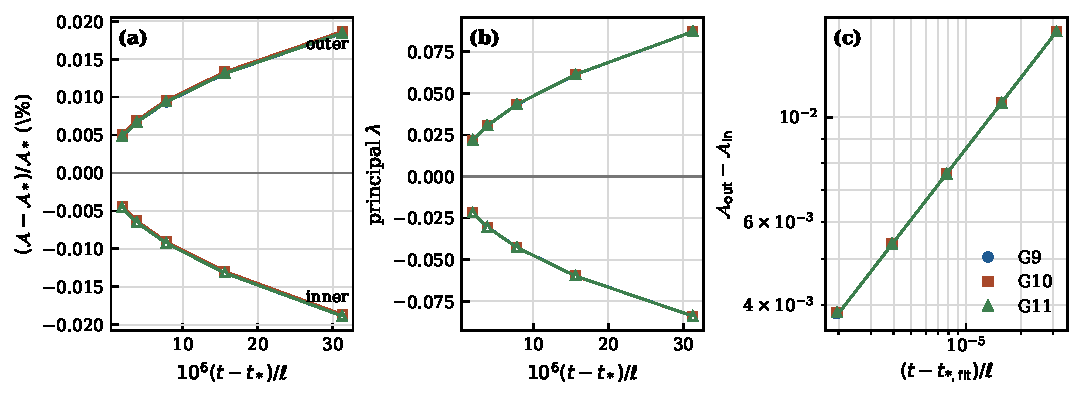
\includegraphics[width=\linewidth]{figures/saddle-node-closure.pdf}
\caption{Three-grid resolution of the free-boundary MOTS saddle-node.
\textbf{(a)} One-sided proper cap area relative to the gridwise near-critical
reference area $\mathcal A_*$ at the selected bracket endpoint, not an exact
critical value; filled symbols denote the outer branch and open symbols the inner branch.
\textbf{(b)} The corresponding principal stability eigenvalues, which approach
zero with opposite signs.  \textbf{(c)} Log--log area separation and the
gridwise fits $\Delta\mathcal A=[s(t-t_{*,\rm fit})]^{1/2}$.}
\label{fig:saddle-node}
\end{figure}

\subsection{Independent half-timestep comparison}

The spatial sequence shares a second-order RK2 step and dense extension, so
its grid agreement alone cannot bound a common temporal bias.  We therefore
reconstructed the G10 parent from $t/\ell=0.001$ to $0.0015$ with
$\Delta t/(2\ell)=1.5625\times10^{-5}$, independently re-solved both endpoint
anchors, replayed the full half-step trajectory, and repeated the continuation,
stability, coefficient, and area-scaling calculations.  Table~\ref{tab:temporal-closure}
shows the direct comparison.  All criteria were fixed before the half-step
result was examined.

\begin{table*}[t]
\centering
\caption{G10 half-timestep comparison.  The $t_*$ entries are bracket
midpoints; their difference is not an uncertainty estimate.  Differences for
$\mathcal A_{\rm nc}$, $a$, and $b$ are relative; $\mathcal A_{\rm nc}$ is the
selected near-critical reference area.}
\label{tab:temporal-closure}
\begin{tabular}{@{}lrrr@{}}
\toprule
quantity & $\Delta t/\ell$ & $\Delta t/(2\ell)$ & difference \\
\midrule
$t_*/\ell$ & $0.0011725452$ & $0.0011725443$ & $9.17\times10^{-10}$ \\
$\mathcal A_{\rm nc}$ & $40.703366$ & $40.703400$ & $8.45\times10^{-7}$ \\
$a$ & $-20.76565$ & $-20.76535$ & $1.42\times10^{-5}$ \\
$b$ & $2.80410$ & $2.80435$ & $9.23\times10^{-5}$ \\
free exponent $p$ & $0.49597$ & $0.49806$ & --- \\
$R^2$ for squared-area fit & $0.9999804$ & $0.9999951$ & --- \\
zero-bracket width & $1.72\times10^{-7}$ & $1.79\times10^{-7}$ & --- \\
\bottomrule
\end{tabular}
\end{table*}

The full- and half-step critical-time brackets overlap.  Their midpoint shift
is $9.17\times10^{-10}$, while the brackets themselves remain approximately
$1.8\times10^{-7}$ wide; the midpoint shift is therefore not interpreted as
the uncertainty in $t_*$.  The half-step run retains the isolated
near-critical principal mode, coefficient signs, and
square-root scaling.  The measured changes satisfy the prospective ceilings:
$\Delta t/64$ for the bracket-midpoint shift, $1\%$ for the near-critical
area, and $20\%$ for each coefficient.  The prescribed decision rule therefore
strongly constrains the shared temporal-discretization concern without
triggering a quarter-step calculation.
Although this is not a separate convergence study of constraint violation,
the complete half-step evolution independently passes the same native
constraint and boundary gates while reproducing the critical observables.
It therefore supplies an indirect temporal check against systematic evolution
error rather than only a continuation-level comparison.
The prospective temporal criteria and full comparison record are reported in
the Supplemental Material \cite{SupplementalMaterial}.

\subsection{Near-critical mode, nondegeneracy, and invariant scaling}

Table~\ref{tab:critical-structure} gives the near-critical diagnostics.  The
representative profile is the smaller-magnitude endpoint of the final
opposite-sign bracket, so its listed eigenvalue need not vanish identically.
At those representatives, $|\lambda|$ lies between
$7.4\times10^{-4}$ and $1.7\times10^{-3}$.  The next eigenvalue in the
$SO(3)$-reduced discretization remains near $5.566$, leaving a large
reduced-sector spectral gap.  The principal right mode is real and
sign-definite.  The unit left--right overlap is imposed by the normalization
above and is not counted as independent evidence.

\begin{table*}[t]
\centering
\caption{Near-critical discrete normal-form observables.  Coefficients are
evaluated at the smaller-magnitude endpoint of the final zero bracket; the
final entries of the two-step evaluations are shown.}
\label{tab:critical-structure}
\begin{tabular}{@{}lrrr@{}}
\toprule
quantity & G9 & G10 & G11 \\
\midrule
next reduced-sector eigenvalue & $5.56598$ & $5.56531$ & $5.56595$ \\
near-critical transversality $a$ & $-20.76513$ & $-20.76565$ & $-20.76493$ \\
near-critical quadratic coefficient $b$ & $2.80717$ & $2.80410$ & $2.81060$ \\
square-root exponent $p$ & $0.4959$ & $0.4960$ & $0.4960$ \\
$R^2$ for $(\Delta\mathcal A)^2$ fit & $0.9999801$ & $0.9999804$ & $0.9999803$ \\
\bottomrule
\end{tabular}
\end{table*}

The centered step-halving evaluations of Eq.~\eqref{eq:normal-form-coefficients}
retain $a<0$ and $b>0$ on every grid.
Adjacent relative differences are at most $3.46\times10^{-5}$ for $a$ and
$2.32\times10^{-3}$ for $b$, compared with the prospective $0.20$ ceilings.
Together, the isolated near-critical principal mode and its bracketed zero
crossing are consistent with a simple critical kernel; the temporal crossing
is transverse and the quadratic term is resolved and nonzero under the stated
discrete convention.  Independently, five paired
fixed-time solves per grid give
\begin{equation}
\mathcal A_{\rm out}-\mathcal A_{\rm in}\propto(t-t_*)^p,
\qquad p\simeq0.496
\label{eq:square-root-scaling}
\end{equation}
Equation~\eqref{eq:square-root-scaling} holds on the three-grid sequence, and
$p\simeq0.498$ in the half-step G10 run.  The
quoted $R^2=0.9999801$--$0.9999804$ belongs to the linear fit of
$(\Delta\mathcal A)^2$ against time, not to the separate free-exponent fit.
Fixing $t_*$ to the continuation midpoint gives $p=0.4951$--$0.4964$; omitting
one of the five offsets gives $p=0.4919$--$0.4996$.  A fixed $p=1/2$ fit has
maximum relative residual $0.9$--$1.2\%$.  These sensitivity checks support a
near-one-half law but do not justify treating the last exponent digits as an
uncertainty estimate.  The shift from $p\simeq0.496$ at the full step to
$p\simeq0.498$ at the half step is toward one-half, consistent with a residual
temporal-discretization bias rather than a fit-selection artifact; two time
steps are not used to infer an error order.  The continuation, operator,
discrete-adjoint, and
invariant-geometry tests therefore identify the local saddle-node structure
through mutually distinct observables.

\section{Interpretation}

The result is a boundary-sensitive test of the local MOTS bifurcation
framework, not simply another observation of pair formation.  The physical
contact condition is part of the nonlinear map in
Eq.~\eqref{eq:free-boundary-map}; its linearization fixes the Robin domain,
the endpoint-eliminated discrete kernel, and the corresponding discrete
adjoint projection.  The
branches are
connected by pseudo-arclength continuation; an isolated near-critical
principal mode accompanies the bracketed zero crossing; both
discrete adjoint nondegeneracy projections are nonzero;
and an invariant geometric separation has the expected one-half exponent.
None of these ingredients is inferred from the branch count alone.  Their
agreement across three spacetime grids and the independent half-timestep G10
comparison support a numerical free-boundary MOTS saddle-node at finite
resolution in the imposed $SO(3)$-symmetric problem.

This chain also supplies a portable diagnostic for other physical-boundary
MOTS problems: formulate the contact condition as part of the boundary-value
map, continue through the singular point, resolve the left and right critical
modes, test the two nondegeneracy projections, and confirm the predicted law
with an invariant geometric observable.  The present calculation establishes
that chain only for the stated discretized evolution; it does not prove that
every free-boundary MOTS problem has the same unfolding.  This single
realization establishes non-obstruction in the tested surface class, not
genericity across free-boundary MOTS problems.

The concrete physical significance lies in the surface class and arena.
The MOTSs terminate orthogonally on a brane inside an explicitly stabilized
compact interval.  They are not imposed as static horizons and are not
continued from a pre-existing connected black string.  Their appearance is
consistent with the local paired-MOTS mechanism under the physical Robin
boundary condition in the tested nonlinear evolution.  The saddle-node mechanism itself
is established theory; the contribution here is resolving its critical
structure in a dynamical brane-terminating problem.

\section{Limitations and boundary of inference}

The initial null result is bounded by the stated launch interval, seed family,
and searched surface classes.  MOTSs depend on slicing; no repaired-line gauge
family is surveyed here.  The critical time is a finite-resolution
continuation estimate in the chosen foliation.  The half-timestep comparison
constrains the common temporal bias, but the nonmonotone three-grid scatter is
not promoted to a continuum theorem, Richardson order, or formal uncertainty
interval.  Equivariance and uniqueness place the principal mode in the
$SO(3)$-invariant sector, but the nonprincipal spectral-gap statement and the
discrete normal-form evaluation remain tied to the symmetric branch and stated
discretization.  They are numerical results, not analytic Fredholm bounds on
the uncomputed nonsymmetric nonprincipal spectrum.  Separately solved
larger-domain parents do not define the same universal formation datum.
Finally, no event horizon, common horizon, global topology change, or
nonlinear stability theorem follows from the evidence.
The archived negative, failed, and incomplete studies underlying these bounds
are summarized in the Supplemental Material \cite{SupplementalMaterial}.

These are not withheld conclusions from the same calculation.  Each requires
a different observable or a different global construction.

\section{Conclusion}

We have numerically verified the local fold hypotheses for a dynamical
free-boundary MOTS saddle-node.  The physical contact condition enters the
boundary-value map and the endpoint-eliminated discrete adjoint projection,
while the ambient geometry is
generated by a nonlinear five-dimensional evolution.  In the concrete
Goldberger--Wise-stabilized braneworld realization, an independently
constructed parent sequence evolves from no accepted capped surface to two
opposite-stability branches on G9, G10, and G11.  Pseudo-arclength continuation
connects them through a grid-consistent critical surface.  The isolated
near-critical principal mode and bracketed zero crossing are consistent with
a simple critical kernel; the discrete adjoint
transversality and quadratic coefficients are nonzero under the stated
discrete normalization, and the invariant proper-area separation follows a
near-one-half law.  An independent G10 half-timestep evolution strongly
constrains the shared temporal-discretization concern.  The repaired-line residual,
operator-resolution, physical-boundary, and deterministic-replay controls
support the formation and critical-structure result.  The calculation therefore advances from
observing post-formation branch anatomy to numerically resolving the local
critical structure of a dynamical free-boundary MOTS problem and provides a
reusable numerical test of the boundary-sensitive normal form.  A separate
future study may use these leaves to investigate a marginal tube or other
global horizon observables; none is claimed here.

\begin{acknowledgments}

I owe a deeply personal debt of gratitude to Chunshan Lin, whose paper
\cite{Lin2026} was the intellectual spark for this project.  Although the
investigation ultimately developed along its own path, the questions raised by
that work made the present study possible.  I am equally and deeply grateful
to Hazel HB, whose steadfast support, patience, and encouragement sustained me
throughout a long and demanding research process.

OpenAI ChatGPT 5.3 and OpenAI Codex (GPT-5 series, accessed August 2026) also
assisted with literature organization and manuscript drafting and revision.
The author checked the cited sources and assumes full responsibility for the
accuracy, interpretation, and final text.
\end{acknowledgments}

\section*{Data Availability}

Machine-readable results, frozen protocols, source manifests, tests, and the
scripts supporting the figures are archived in the published Zenodo version
identified by
\href{https://doi.org/10.5281/zenodo.22087164}{doi:10.5281/zenodo.22087164}.
The complete version series is identified by the concept DOI
\href{https://doi.org/10.5281/zenodo.22085054}{doi:10.5281/zenodo.22085054}.
The version-controlled Python source, frozen protocol implementations, and
test suite are publicly available in the
\href{https://github.com/RonBibb/free-boundary-mots-saddle-node}{GitHub repository}.
The Zenodo record is the citable archival authority for the scientific
results.

\bibliographystyle{apsrev4-2}
\bibliography{references}

\end{document}
